    
                %\title{LaTeX Portrait Poster Template}
%%%%%%%%%%%%%%%%%%%%%%%%%%%%%%%%%%%%%%%%%
% a0poster Portrait Poster
% LaTeX Template
% Version 1.0 (22/06/13)
%
% The a0poster class was created by:
% Gerlinde Kettl and Matthias Weiser (tex@kettl.de)
% 
% This template has been downloaded from:
% http://www.LaTeXTemplates.com
%
% License:
% CC BY-NC-SA 3.0 (http://creativecommons.org/licenses/by-nc-sa/3.0/)
%
%%%%%%%%%%%%%%%%%%%%%%%%%%%%%%%%%%%%%%%%%

%----------------------------------------------------------------------------------------
%   PACKAGES AND OTHER DOCUMENT CONFIGURATIONS
%----------------------------------------------------------------------------------------

\documentclass[a0,portrait]{a0poster}
\usepackage[dutch]{babel}
\usepackage{enumitem}
\usepackage{apacite}
\usepackage{multicol} % This is so we can have multiple columns of text side-by-side
\columnsep=100pt % This is the amount of white space between the columns in the poster
\columnseprule=3pt % This is the thickness of the black line between the columns in the poster

\usepackage[svgnames]{xcolor} % Specify colors by their 'svgnames', for a full list of all colors available see here: http://www.latextemplates.com/svgnames-colors

\usepackage{times} % Use the times font
%\usepackage{palatino} % Uncomment to use the Palatino font

\usepackage{graphicx} % Required for including images
\usepackage{booktabs} % Top and bottom rules for table
\usepackage[font=small,labelfont=bf]{caption} % Required for specifying captions to tables and figures
\usepackage{amsfonts, amsmath, amsthm, amssymb} % For math fonts, symbols and environments
\usepackage{wrapfig} % Allows wrapping text around tables and figures

\begin{document}

%----------------------------------------------------------------------------------------
%   POSTER HEADER 
%----------------------------------------------------------------------------------------

% The header is divided into two boxes:
% The first is 75% wide and houses the title, subtitle, names, university/organization and contact information
% The second is 25% wide and houses a logo for your university/organization or a photo of you
% The widths of these boxes can be easily edited to accommodate your content as you see fit

\begin{minipage}[b]{0.75\linewidth}
\VeryHuge \color{NavyBlue} \textbf{Bewustzijn heeft aandacht nodig} \color{Black}\\ % Title
\Huge\textit{Gistperceptie onder dualtaskcondities}\\[2.4cm] % Subtitle
\huge \textbf{Raoul Grouls\textsuperscript{1},
	\,Libby van den Besselaar\textsuperscript{2},
	\,Eva Bakels\textsuperscript{3},
	\,Kiki Piekartz\textsuperscript{4}}\\[0.5cm] % Author(s)
\huge Universiteit Utrecht,\,Kunstmatige Intelligentie,\, Nederland\\[0.4cm] % University/organization
\normalsize \texttt{1: r.h.grouls@students.uu.nl}\\
\texttt{2: l.l.m.vandenbesselaar@students.uu.n}\\
\texttt{3: e.e.bakels@students.uu.nl}\\
\texttt{4: k.g.piekartz@students.uu.nl}\\
\end{minipage}
%
\begin{minipage}[b]{0.3\linewidth}

\includegraphics[width=20cm]{uu-logo.png}\\ 
\end{minipage}

\vspace{1cm} % A bit of extra whitespace between the header and poster content

%----------------------------------------------------------------------------------------

\begin{multicols}{3} % This is how many columns your poster will be broken into, a portrait poster is generally split into 2 columns

%----------------------------------------------------------------------------------------
%   ABSTRACT
%----------------------------------------------------------------------------------------

\color{Navy} % Navy color for the abstract

\begin{abstract}
bla die bla
\end{abstract}
%----------------------------------------------------------------------------------------
%   INTRODUCTION
%----------------------------------------------------------------------------------------

\color{Black} % SaddleBrown color for the introduction
\section*{Introductie}
Algeria is situated in \cite{Block_2011} northern Africa, bordering the Mediterranean Sea, between Morocco and Tunisia. Algeria has the 9th-largest reserves of natural gas in the world. It ranks 16th in proved oil reserves.  
\begin{itemize}
\item Geothermal exploration program started in 1967 by National Oil Comapny SONATRACH.
\item From 1983 onwards the geothermal research has been continued by the Renewable Energies Center of Algeria.
\end{itemize}

\color{Black} % DarkSlateGray color for the rest of the content

\section*{Hypothese}
The geology of Algeria (Figure 1) is divided into two main structural units: the folded Tellian Domain in the North, and the Saharian Platform in the South.
\begin{center}\vspace{1cm}
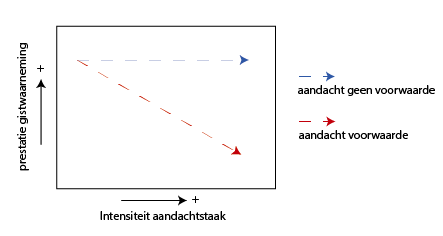
\includegraphics[width=1.0\linewidth]{illustratieHypothese.png}
\captionof{figure}{\color{Green} Major geotectonics units of West Africa modified from Fabre. 1: Tertiary and Quaternary; 2: Alpine molasses; 3: Tertiary thrust sheet; 4: Secondary tabular; 5: Secondary plicative; 6: Primary plicative; 7: Primary tabular; 8: Precambrian and Precorce Cambrian of Sahara; 9: Cenozoic magma; 10: Megafault.}
\end{center}%\vspace{1cm}
%----------------------------------------------------------------------------------------
%   GEOTHERMAL DATA
%----------------------------------------------------------------------------------------
\section*{Methode}
\subsection*{Demografie}
\begin{tabular}{r r r r r r}
	\hline
	med. leeftijd & SD leeftijd & min. leeftijd & max. leeftijd & man/vrouw & n\\
	\hline
	22 & 15 & 17 & 60 & 0.5 & 34\\
	\hline
\end{tabular}
\begin{center}\vspace{1cm}
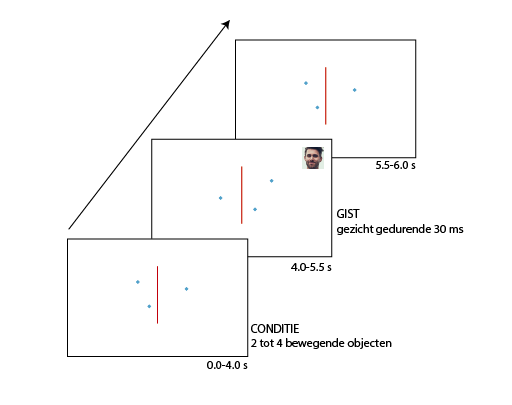
\includegraphics[width=1.0\linewidth]{Methode.png}
\captionof{figure}{\color{Green} (A) Temp. vs. depth for different regions.}
\end{center}\vspace{1cm}

%------------------------------------------------

\subsection*{Resultaten}
\begin{enumerate}
\item The Tlemcenian dolomites in the NW-Algeria: thermal waters are related to the Plio-Quaternary volcanic rocks; bicarbonate water type.
\item Carbonate formations in the NE-Algeria: area is 15,000 km$^2$; high flow rates (\textgreater100 L/s); highest temperature in Algeria (98 $^{\circ}$C). 
\end{enumerate}

\subsection*{Hot Springs}
\begin{center}\vspace{1cm}
	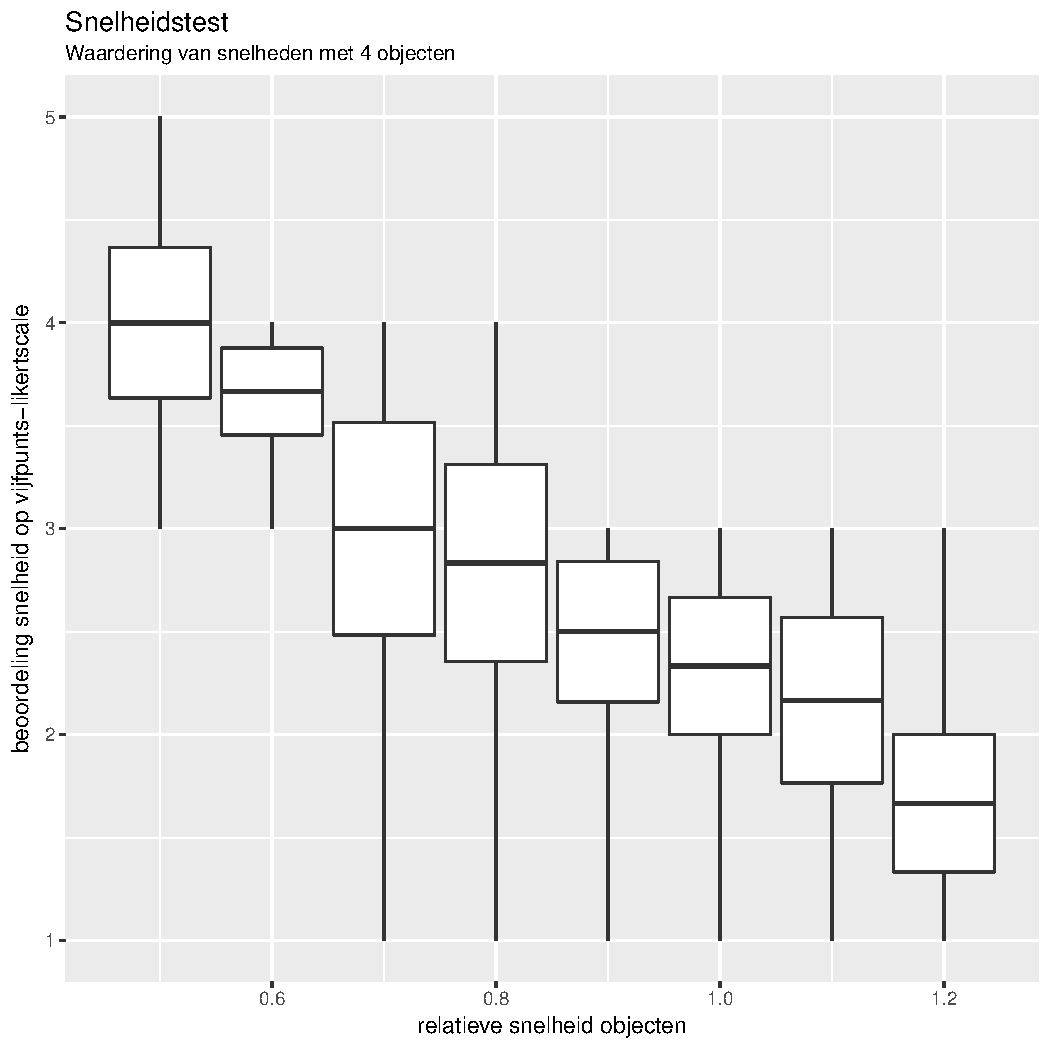
\includegraphics[width=0.5\linewidth]{boxplot-snelheidstest.pdf}
	\captionof{figure}{\color{Green} Temperatures of the main hot springs of the northern part of Algeria}
\end{center}\vspace{1cm}

\begin{center}\vspace{1cm}
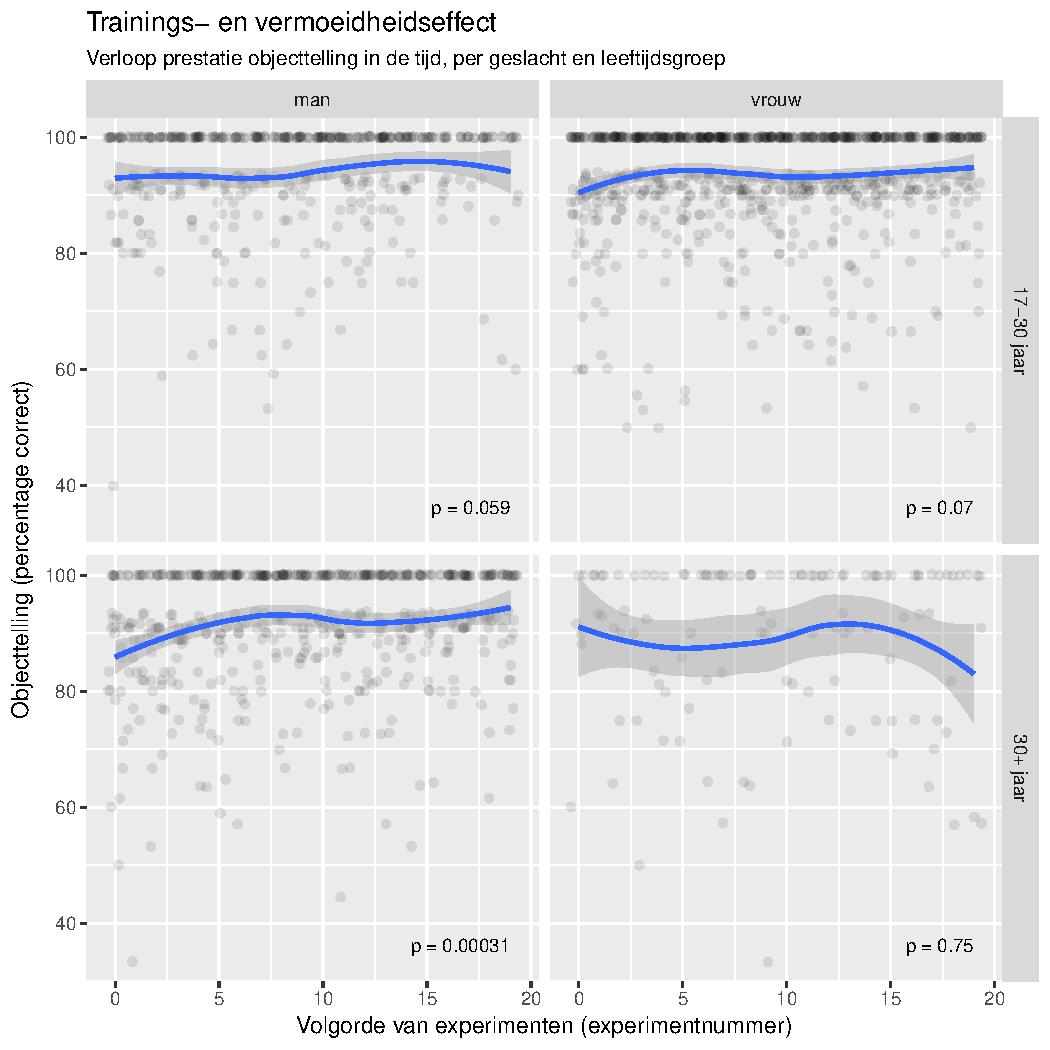
\includegraphics[width=1.0\linewidth]{training-grid.pdf}
\captionof{figure}{\color{Green} Temperatures of the main hot springs of the northern part of Algeria}
\end{center}\vspace{1cm}

\begin{tabular}{r r r}
	\hline
	p & c2 & afkap\\
	\hline
	0.07 & -0.03 & 5\\
	0.03 & -0.03 & 8\\
	0.01 & -0.04 & 9\\
	0.01 & -0.03 & 10\\
	0.04 & -0.02 & 15\\
	0.03 & -0.02 & 17\\
	0.02 & -0.03 & 20\\
	\hline
\end{tabular}

\begin{center}\vspace{1cm}
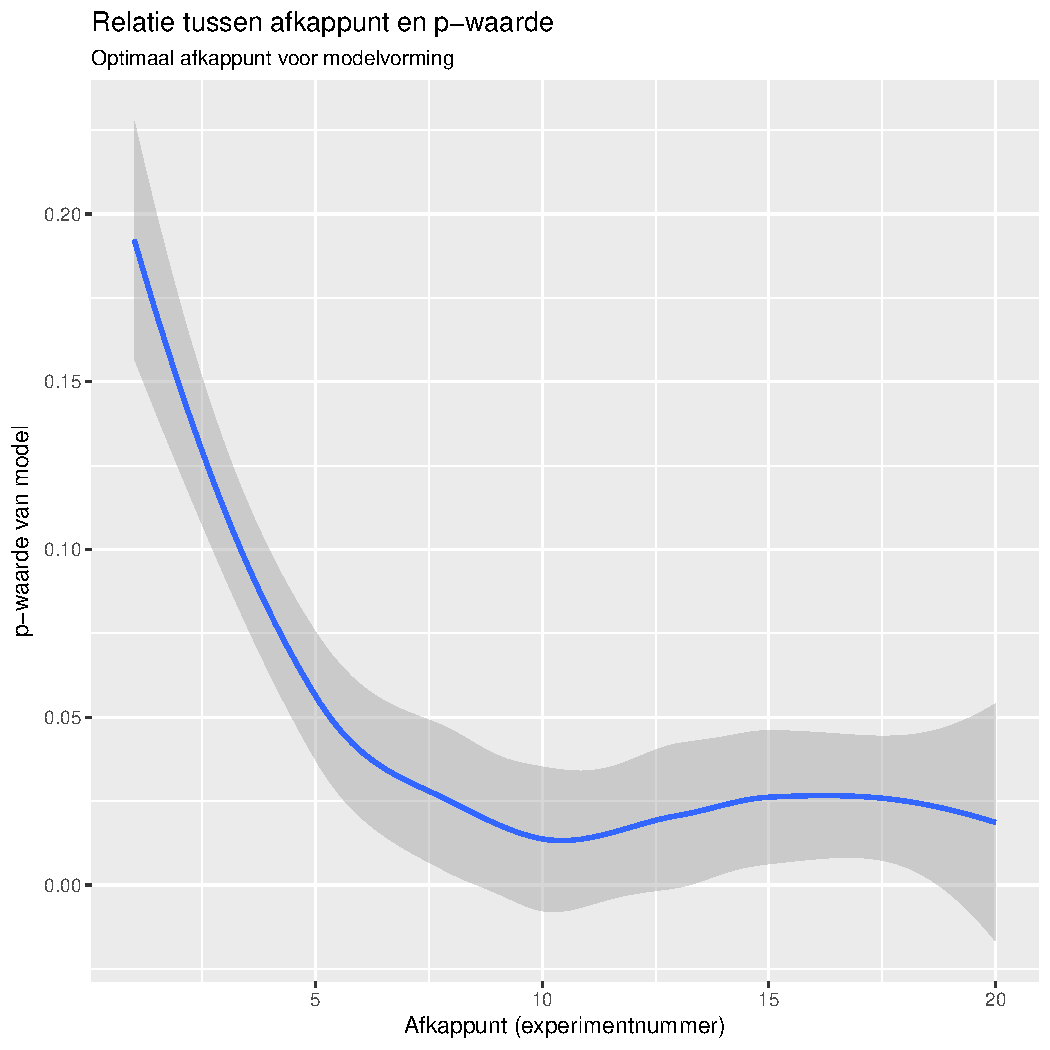
\includegraphics[width=0.8\linewidth]{pwaardes.pdf}
\captionof{figure}{\color{Green} Total Dissolved Solid (TDS) of the main hot springs of the northern part of Algeria}
\end{center}\vspace{1cm}

\begin{center}\vspace{1cm}
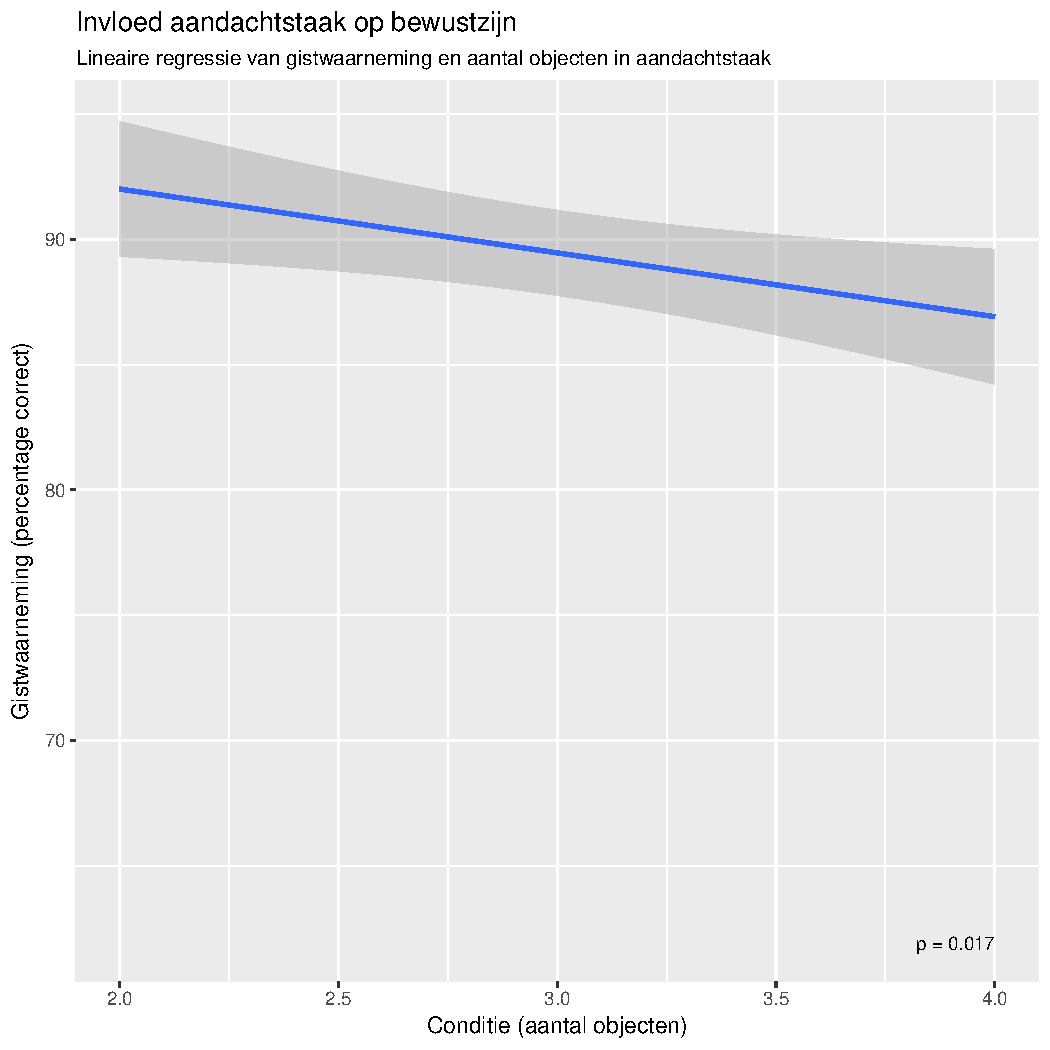
\includegraphics[width=1.0\linewidth]{lineaireRegressie.pdf}
\captionof{figure}{\color{Green} (A) Mixing model to illustrate the relative contribution of magmatic, meteoric and crustal sources of gases in NE Algerian geothermal discharges. (B) Photo of the concretions of Hammam Meskhoutine (NE Algeria). The height of the concretions on successive conduits reaches 30 m.}
\end{center}\vspace{1cm}

\subsection*{Discussie}
\begin{itemize}
\item Utilizations of the hot water in Algeria are balneology, space and greenhouse heating. 
\item Heat-pump in a primary school (NW Algeria) for heating and cooling purposes.
\item Tilapia fish farming in south of Algeria (Ghardaia and Ouargla).
\item Greenhouses for melon and tomato cultivation in South of Algeria (Ouargla and Touggourt).
\item Future projects: binary-cycle geothermal power plant in Guelma (NE-Algeria); heat-pump in Khenchla (NE Algeria).
\end{itemize}
The total energy use for geothermal is about 1,778.65 TJ/yr.

\begin{center}\vspace{1cm}
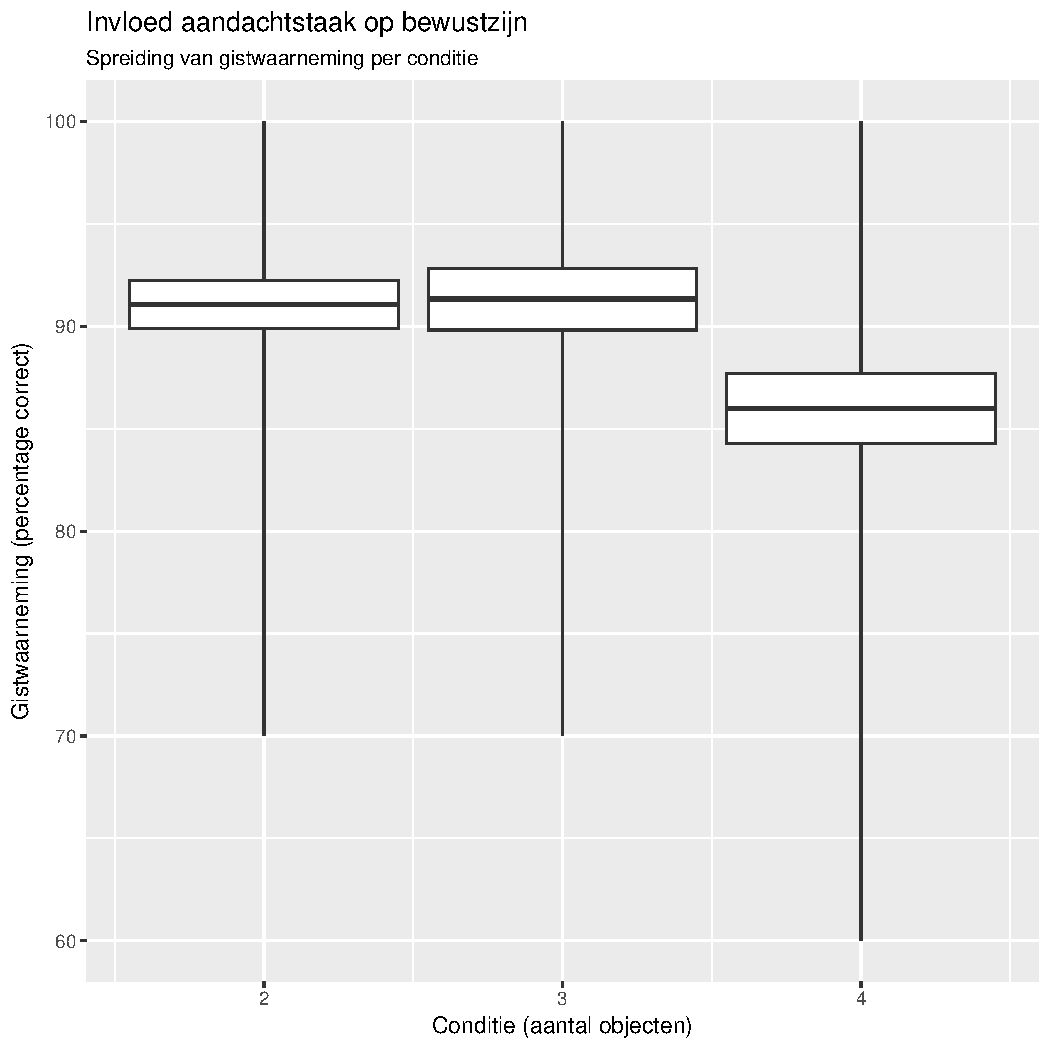
\includegraphics[width=0.8\linewidth]{boxplotGist-conditie.pdf}
\captionof{figure}{\color{Green} Location of Algerian geothermal uses sites}
\end{center}\vspace{1cm}

\subsection*{Geothermal Conceptual Models}
\begin{center}\vspace{1cm}
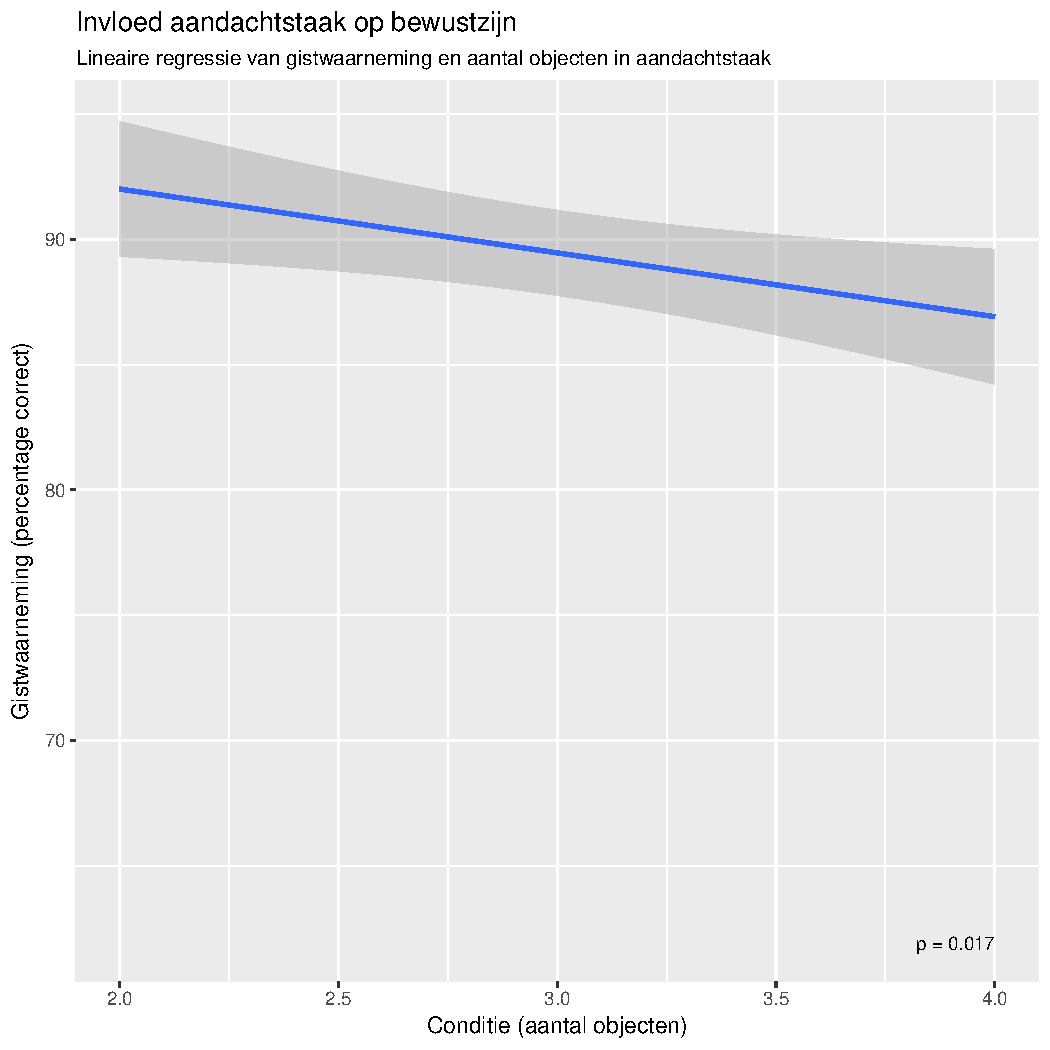
\includegraphics[width=1.0\linewidth]{lineaireRegressie.pdf}
\captionof{figure}{\color{Green} (a) Idealized northern Algerian geothermal system characterized by heating of the filtered meteoric water. (b) Idealized southern Algerian geothermal system, characterized by basement heating of the sedimentary basin}
\end{center}

%----------------------------------------------------------------------------------------
%   CONCLUSIONS
%----------------------------------------------------------------------------------------

\color{SaddleBrown} % SaddleBrown color for the conclusions to make them stand out

\section*{Conclusies}
Despite being a petroleum- and gas-rich country, Algeria is making efforts to exploit its renewable energies. The Algerian government has adopted new renewable energy laws and financial support for the investors to facilitate the exploitation of the renewable energies for electricity production and direct utilizations. Algeria has relatively abundant geothermal resources especially in the northeastern parts but not totally used.
\color{Black} % Set the color back to DarkSlateGray for the rest of the content

%----------------------------------------------------------------------------------------
%   FORTHCOMING RESEARCH
%----------------------------------------------------------------------------------------


 %----------------------------------------------------------------------------------------
%   REFERENCES
%----------------------------------------------------------------------------------------


%----------------------------------------------------------------------------------------
\bibliographystyle{apacite}
\bibliography{biblio} 
\end{multicols}
\end{document}
              
            